\documentclass[a4paper,10pt]{article}

\usepackage{tkz-orm}
\usepackage{pgfmanualstyle}

\usetikzlibrary{fit} % fitting library
\usetikzlibrary{positioning} % for left/right=of ...

\usepackage[colorlinks=false,pdfborder={0 0 0}]{hyperref}
% [pagebackref=true, backref=true, pdfborder={0 0 0}
\usepackage{multirow}

\usepackage{makeidx}
\makeindex

\def\ormVersion{0.1dev}
\def\ormDate{August 2010}
\newif\ifappendix
\appendixfalse
\appendixtrue

% --------------------------------------------------------------
%% Beginning of the documentation
% --------------------------------------------------------------
\title{The \textsf{tkz-orm} package\\Object-Role Model Drawing Library}
\author{Jakob Vo\ss\\{\footnotesize jakob.voss@gbv.de}}
\date{Version \ormVersion\\\ormDate\\[5mm]\url{http://purl.org/net/tkz-orm}}

\begin{document}
\maketitle

\begin{abstract}
This package provides styles for drawing Object-Role Model (ORM)
diagrams in \TeX{} based on the \textsc{pgf} and \tikzname\ picture environment.
\end{abstract}

\tableofcontents
\pagebreak

\section{Introduction}
\label{sec:introduction}

\textsf{tkz-orm} is intended to help you creating Object-Role Model (ORM) diagrams. It is based on the \textsc{pgf} and \tikzname\footnote{\url{http://sourceforge.net/projects/pgf/}} picture macro package for \TeX. and provides additional styles and commands to typeset ORM2 diagrams.\footnote{This version is tested with \tikzname{} version 2.00-cvs 2009-09-04. It will either be backported to \tikzname{} version 2.00 or work with a yet to published new release of \tikzname{}.} With \textsf{tkz-orm} you can ``program'' ORM diagrams just as you ``program'' your document when you use \LaTeX\ -- including the inherental lack of \textsc{wysiwyg}. Unless multi-touch e-paper interfaces become usable, \textsf{tkz-orm} can best be combined with a whiteboard or paper and pencil --- but you may also find ways to automatically create ORM diagrams with \textsf{tkz-orm}.

\subsection*{Status of this package}
This is the first public version of \textsf{tkz-orm}. Please send your comments to the author so the package can be improved. All parts of the package are available at least under the \LaTeX{} Project Public License\cite{LPPL} and the GNU Public license\cite{GPL2}. For details have a look at the file |LICENSE| that is part of this package. The permament URL of \textsf{tkz-orm} is \url{http://purl.org/net/tkz-orm} which redirects you to its current location.

\subsection*{ORM in a nutshell}
Object-Role Modeling (ORM)\footnote{\url{http://www.orm.net/}} is a fact-oriented modeling language that evolved from the \textit{Natural-language Information Analysis Method} (NIAM) by G.M. Nijssen. The current version (ORM2) is mainly based on works of Terry Halpin. Like ERM, UML, and other data modeling languages ORM helps to identify and abstract information objects, relationships, and rules in a Universe of Discourse to be formalized and implemented on another level. ORM includes a graphical notation and a defined verbalization in natural language. Models can further be validated by populating fact tables with sample data. An overview of the ORM2 Graphical Notation is given in \cite{Halpin2005} and more details in \cite{Halpin2008}. An ORM model consists of object types (section~\ref{sec:objecttypes}), $n$-ary predicates  (section~\ref{sec:predicates}). Each of the $n$ roles of an $n$-ary predicate is connected to an object type that plays the specific role in this predicate. Furthermore a model can contain constraints (section~\ref{sec:constraints}), subtypes (section~\ref{sec:subtyping}), and additional features (section~\ref{sec:additionalfeatures}). \textsf{tkz-orm} also allows you to change the appearance of ORM diagrams (section~\ref{sec:generalstyles}).

\begin{figure}[ht]
  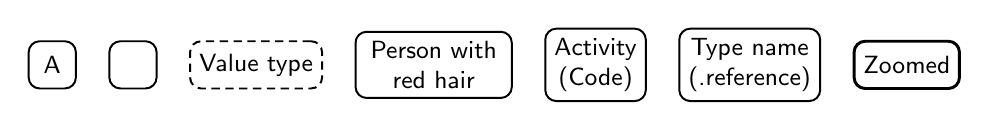
\begin{tikzpicture}
    \entity (A) at (0,0) {A};
    \entity[right=of A] (blank) {};
    \value[right=of blank] (value) {Value type};
    \entity[right=of value,text width=1.75cm] (fixedwidth) {Person with red hair};
    \entity[right=of fixedwidth] (tabular) {Activity\\(Code)};
    \entity[right=of tabular] (typenamelabel) {Type name\\(.reference)};
    \entity[right=of typenamelabel,zoomed] () {Zoomed};
  \end{tikzpicture}
  \caption{Examples of object types in ORM}
\end{figure}

\pagebreak
\section{Object Types}
\label{sec:objecttypes}\index{Object types}\index{Entities}\index{Values}
Object types are drawn as rectangles with rounded corners. The object's type name is written as node text inside. \emph{Entity types} use solid border lines and \emph{value types} use dashed border lines. The minimal size of an object is set to 6mm$\times$6mm. This package provides the following styles for entities and values:

\begin{stylekey}{entity}
This style is to be used with nodes that represent entity types.
\begin{codeexample}[]
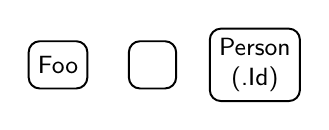
\begin{tikzpicture}
  \node[entity] at (0,0) {Foo};
  \node[entity] (unnamed) at (1.2,0) {};
  \node[entity] at (2.5,0) {Person\\(.Id)};
\end{tikzpicture}
\end{codeexample}
\end{stylekey}

\begin{stylekey}{value}
This style is to be used with nodes that represent value types.
\begin{codeexample}[]
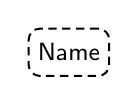
\begin{tikzpicture}
  \node[value] {Name};
\end{tikzpicture}
\end{codeexample}
\end{stylekey}

\begin{stylekey}{every entity}
\stylekeyheadline{every value}
Each of this styles is envoked by the styles |entity| or |value|. Change one of this styles to change the appearance of entity or value types.
\begin{codeexample}[width=3cm]
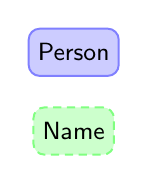
\begin{tikzpicture}[
  every entity/.style={draw=blue!50,fill=blue!20},
  every value/.style={draw=green!50,fill=green!20}]
  \node[entity] (P) at (0,0) {Person};
  \node[value]  (N) at (0,-1) {Name};
\end{tikzpicture}
\end{codeexample}
\end{stylekey}

\begin{stylekey}{every object type}
  This style is envoked by the styles |entity| and |value|. Change this style to change the common appearance of entity and value types.
\begin{codeexample}[width=3cm]
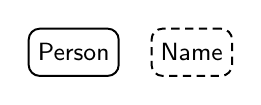
\begin{tikzpicture}[
  every object type/.style={shape=circle}]
  \node[entity] (P) at (0,0) {Person};
  \node[value]  (N) at (1.5,0) {Name};
\end{tikzpicture}
\end{codeexample}
\end{stylekey}

\noindent
Since entity types and value types are very frequent node types in an ORM diagram, there are two special abbreviations for creating object types:

\begin{command}{entity}
Inside |{tikzpicture}| this is an abbreviation for |\node[entity]|.
\end{command}

\begin{command}{value}
Inside |{tikzpicture}| this is an abbreviation for |\node[value]|.
\end{command}



\section{Predicates and Roles}
\label{sec:predicates}\index{predicates}\index{roles}
The relationship parts (\emph{roles}) played by objects are shown as boxes of fixed size (4mm$\times$2.5mm). A \emph{predicate} is a sequence of one or more concatenated role boxes. Predicates can be created with the following styles:

\begin{stylekey}[\opt{\meta{number of roles}}]{roles}
\stylekeyheadline[ (alias for \texttt{roles=1})]{role}
Shapes the current node as predicate with a given number of role boxes. Numbers from 1 to 20 are supported. The default value is 2 (binary).

\begin{codeexample}[]
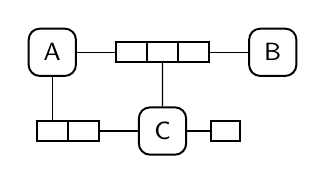
\begin{tikzpicture}[orm]
  \entity (A) {A};
  \entity (B) at (2.8,0) {B}
          edge node[roles=3] (p) {} (A);
  \entity (C) at (1.4,-1) {C}
          edge (p.south);
  \node[role] at (2.2,-1){} edge (C);
  \draw (A) |- node[roles,xshift=2mm]{} (C);
\end{tikzpicture}
\end{codeexample}
\end{stylekey} % roles

\begin{stylekey}[\opt{\meta{number of roles}}]{vroles}
\stylekeyheadline[ (alias for \texttt{vroles=1})]{vrole}
Shapes the current node as predicate rotated by 90 degree (vertical).
\end{stylekey} % vroles

\begin{stylekey}{relation}
  \stylekeyheadline[]{relationship}
  This styles are to be used with connection lines between objects and roles. By default it just sets the line width to 0.25mm by including the style |every orm line|. Alternatively of using this style you can enable the general style |orm| (see section~\ref{sec:generalstyles}) and just draw a normal line.
\begin{codeexample}[width=3cm]
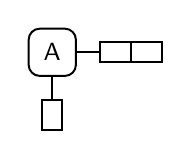
\begin{tikzpicture}
  \node[entity] (A) {A};
  \node[roles] (r) at (1,0) {};
  \draw[relation] (A) -- (r);
  \node[vrole] at (0,-.8){} edge[relation] (A);
\end{tikzpicture}
\end{codeexample}
\end{stylekey}

\noindent
Table~\ref{tab:roleabbr} lists abbreviations that can be used for creating predicate nodes and relationship lines inside |{tikzpicture}|.

\begin{table}[h]
\begin{tabular}{lll}
\textbf{Command(s)} & \textbf{Abbreviation for} & \\
\commandentry{unary} or \commandentry{role} & |\node[role]| & 
  \colorbox{graphicbackground}{\tikz \unary{};} \\
\commandentry{binary} or \commandentry{roles} & |\node[roles]| &
  \colorbox{graphicbackground}{\tikz \binary{};} \\
\commandentry{ternary} & |\node[roles=3]| &
  \colorbox{graphicbackground}{\tikz \ternary{};} \\
\commandentry{vunary} or \commandentry{vrole} & |\node[vrole]| &
 \multirow{3}{2cm}{\colorbox{graphicbackground}{
   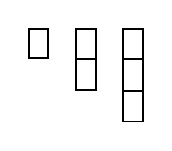
\begin{tikzpicture}
    \vunary at (0,0){} ;
    \vbinary at (0.6,-0.2){};
    \vternary at (1.2,-0.4){};
   \end{tikzpicture}
 }} \\
\commandentry{vbinary} or \commandentry{vroles} & |\node[vroles]| \\
\commandentry{vternary} & |\node[vroles=3]| \\
\commandentry{plays} & |\draw[relationship]| &
  \colorbox{graphicbackground}{\tikz \plays (0,0) -- (1,0);} \\
\end{tabular}
\caption{Abbreviations to create predicates, roles, and relationship lines}
\label{tab:roleabbr}
\end{table}

\noindent The general style of predicates and roles can be modified by the following keys:

\begin{stylekey}{every predicate}
By changing this style you can modify the common appearance of predicates.
\begin{codeexample}[width=3cm]
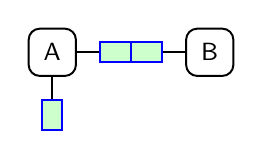
\begin{tikzpicture}[
  every predicate/.style={draw=blue,fill=green!20}]
  \entity at (2,0) (B) {B};
  \entity (A) {A} edge[relation] node[roles]{} (B);
  \vunary at (0,-0.8) (r) {} edge[relation] (A);
\end{tikzpicture}
\end{codeexample}
\end{stylekey}

\begin{stylekey}{every relationship}
  This style is envoked by the style |relationship|. To change the appearance of explicit relationship lines you can change this style. Please keep in mind that nodes placed on a line by |node| in one operation inherit properties from  the line they refer to, so you should create relationship lines with |plays|.
\begin{codeexample}[width=3cm]
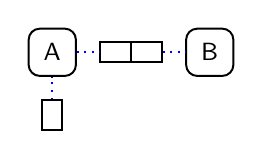
\begin{tikzpicture}[orm,
  every relationship/.style={draw=blue,dotted}]
  \entity (A) {A};
  \binary (r) at (1,0) {};
  \entity (B) at (2,0) {B};
  \plays (A) -- (r) -- (B);
  \vunary at (0,-0.8) (r) {} edge[relation] (A);
\end{tikzpicture}
\end{codeexample}
\end{stylekey}

\noindent
Predicates are drawn either horizontally (|roles|) or vertically (|vroles|) as nodes with one or more parts. Figure~\ref{fig:hanchors} shows some of the anchors. Vertical predicates are rotated by 90 degree so |north| is at the left, |west| is at the bottom etc.
% TODO: define better anchors or anchor aliases (start=west, end=east, top=north, bottom=south, role 1=one north)

\begin{figure}[h]
\centering
\begin{codeexample}[width=10cm]
\Large
\begin{tikzpicture}
  \node[roles=3,shape example,inner ysep=0.75cm] (s) {};
  \foreach \anchor/\placement in
    {one north/below, one south/above,
     three north/below, three south/above,
     one split/below, one split north/above, one split south/below,
     two split/below, two split north/above, two split south/below,
     north/below, south/above, east/below, west/below, center/above,
     north west/above, north east/above, south west/below, south east/below}
    \draw[shift=(s.\anchor)] plot[mark=x] coordinates{(0,0)}
       node[\placement] {\scriptsize\texttt{s.\anchor}};
\end{tikzpicture}
\end{codeexample}
\label{fig:hanchors}
\caption{Node anchors of an ORM predicate}
\end{figure}

\noindent
The verbalization of a predicate can be given as |label| next to a predicate. For binary relationships forward and inverse readings can be seperated by a slash. To show the inverse reading, add an arrow tip with the commands |\ormleft| or |\ormup| (see section~\ref{sec:ormtext}). Labels for predicates with more then two roles must contain three dots (|\ldots|) for each inner role. Role names and indices can be added by different styles.
% TODO: Show how to change label distance with style |label distance| :
% \begin{tikzgraphic}[orm] % needed - there is no "every label/.style={orm}"
% \node[role,label={R}] (r1) {};                    % put the label above
% \node[role,right=of r1,label={below:R}] (r2) {};  % put the label below
% \node[role,right=of r2,label={[label distance=1.5mm]above:{R}},unique] (r3) {};
% \end{tikzgraphic}

\begin{figure}[h]
\centering
\begin{codeexample}[]
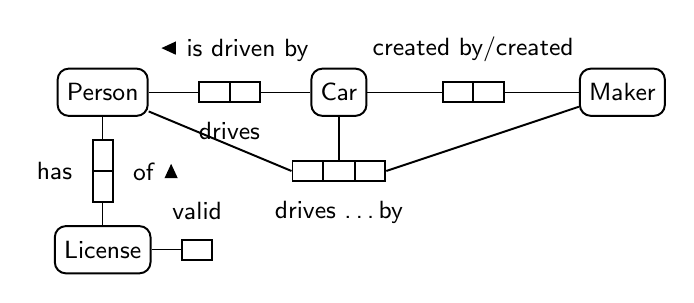
\begin{tikzpicture}[orm]
  \entity at (0,2) (P) {Person};
  \entity at (3,2) (C) {Car};
  \entity at (0,0) (L) {License};
  \entity at (6.6,2) (M) {Maker};
  \unary[label=valid] at (1.2,0) (V) {} edge (L);
  \draw (P) to node[roles,
         label=below:drives,label=\ormleft{is driven by}]{} (C);
  \draw (P) to node[vroles,label=has,label=below:\ormup{of}]{} (L);
  \draw (C) to node[roles,label=created by/created]{} (M);
  \ternary[label=below:drives \ldots by] at (3,1) (t) {};
  \plays (P) -- (t.west);
  \plays (C) -- (t);
  \plays (M) -- (t.east);
\end{tikzpicture}
\end{codeexample}
\end{figure}

\begin{stylekey}{role name}
This style is to be used with role names. Role names can be displayed in square brackets and blue color next to a role box. % TODO: add role name as 'label' style
\begin{codeexample}[width=3cm]
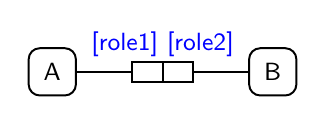
\begin{tikzpicture}[orm]
  \entity (A) at (0,0) {A};
  \entity (B) at (2.8,0) {B};
  \plays (A) edge node(r)[roles]{} (B);
  \node[role name,
     at=(r.north),anchor=south east] {[role1]};
  \node[role name,
     at=(r.north),anchor=south west] {[role2]};
\end{tikzpicture}
\end{codeexample}
\end{stylekey}

\begin{stylekey}[\meta{n}\opt{\texttt{:}\meta{index}}]{index}
Adds a role index as small label at the $n$th role box (default: $n$).
\begin{codeexample}[]
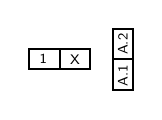
\begin{tikzpicture}
\binary[index=1,index=2:X] {};
\vroles[index=A.1,index=2:A.2] at (.8,0) {};
\end{tikzpicture}
\end{codeexample}
\end{stylekey}


\section{Constraints}
\label{sec:constraints}\index{Constraints}
ORM provides a rich set of constraints: Mandatory constraints (section~\ref{sec:mandatoryconstraints}) and uniqueness constraints (section~\ref{sec:uniquenessconstraints}) limit the way objects can be combined in predicates. External constraints (section~\ref{sec:externalconstraints}) and subtype constraints (section~\ref{sec:subtyping}) involve multiple roles or object types. All constraints are displayed in violet color and either drawn directly at an object type or role, or linked to one or more object types or role with dotted or dashed lines or arrows (see the styles |limits| and |limits to|). ORM2 defines a set of symbols for external (section~\ref{sec:externalconstraints}), ring (section~\ref{sec:ringconstraints}) and other types of constraints. The general \textsc{tkz-orm} constraint key |constraint| only sets the font to violet. An optional key value can be used to add a predefined constraint symbol at the current position.


\subsection{Uniqueness Constraints}
\label{sec:uniquenessconstraints}
By default every row in a fact table is unique. To express additional uniqueness constraints on one or more roles of a fact table or to explicitly express the uniqueness on the full predicate, a \emph{uniqueness bar} is drawn above or below the fact roles. If the bar spans two or more non-adjacent roles, it is drawn as dotted line above or below the excluded roles. Bars can be stacked in multiple levels. To draw uniqueness bars you can use the following styles at predicate nodes:

\begin{stylekey}[\opt{\meta{from}\texttt{-}\meta{to}\texttt{:}\meta{level}}]{unique}
Draws a uniqueness constraint bar above one or more roles. All parts of the key value are optional. As default a simple uniqueness bar above (\meta{level}|=1|) the first role (\meta{from}|=1|) is drawn. To make a bar span multiple roles, use the \meta{from}|-|\meta{to} syntax. Negative levels drawn the bar below the roles.
\begin{codeexample}[]
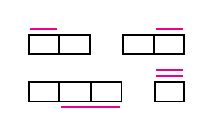
\begin{tikzpicture}
\binary[unique] at (0,0) {};
\binary[unique=2] at (1.2,0) {};
\ternary[unique=2-3:-1] at (0.2,-0.6) {};
\unary[unique=1,unique=1:2] at (1.4,-0.6) {};
\end{tikzpicture}
\end{codeexample}
\end{stylekey}

\begin{stylekey}[\opt{\meta{from}\texttt{-}\meta{to}\texttt{:}\meta{level}}]{skip unique}
Draws a dotted uniqueness constraint bar. The syntax is the same as at the |unique| key.
The bar includes background color in the gaps between dots, so it can be drawn on top of 
another bar.
\begin{codeexample}[]
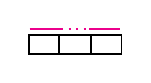
\begin{tikzpicture}
\ternary[unique=1-3,skip unique=2] {};
\end{tikzpicture}
\end{codeexample}
\end{stylekey}

\begin{stylekey}{uniqueness bar}
\stylekeyheadline[]{skipped uniqueness bar}
This styles can be used to draw a line in the same style as a uniqueness constraint bar or a dotted uniqueness constraint bar.
\begin{codeexample}[width=3cm]
\tikz\draw[uniqueness bar] (0,0) -- (2,0);
\end{codeexample}
\begin{codeexample}[width=3cm]
\tikz\draw[skipped uniqueness bar] (0,0) -- (2,0);
\end{codeexample}
\end{stylekey}

\noindent
Please note that elementary $n$-ary predicates should only have uniqueness constraints of at least $n-1$ roles. Picture~\ref{fig:splitternary} shows how to split a ternary predicate with unique constraint bar on one role.

\begin{figure}[h]
\centering
\begin{codeexample}[]
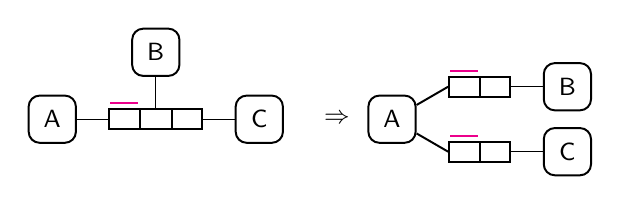
\begin{tikzpicture}[orm] % needs positioning library
  \ternary[unique] (t) at (0,0) {};
  \entity[left=of t]  {A} edge (t);
  \entity[above=of t] {B} edge (t);
  \entity[right=of t] {C} edge (t);
  \node at (2.3,0) {$\Rightarrow$};
  \entity (A) at (3,0) {A};
  \binary[right=of A.north east,yshift=1mm,unique] (t1) {};
  \binary[right=of A.south east,yshift=-1mm,unique] (t2) {};
  \plays (A) -- (t1.west); \plays (A) -- (t2.west);
  \entity[right=of t1] {B} edge (t1);
  \entity[right=of t2] {C} edge (t2);
\end{tikzpicture}
\end{codeexample}
\caption{A ternary predicate can be split into to binary predicates}
\label{fig:splitternary}
\end{figure}


\subsection{Mandatory Role Constraints}
\label{sec:mandatoryconstraints}
To indicate explicitly that a role is mandatory, a mandatory role dot is added to either end of the line that connects the role to its object. Usually it is placed at the object type end. This package defines the style key |constraint dot| (alias |cdot|) and the following keys which can be used to add mandatory role dots to lines drawn with the |to| operation.

\begin{stylekey}{constraint dot}
\stylekeyheadline[]{cdot}
Draws the current node as mandatory role dot.
\begin{codeexample}[]
\tikz \node[cdot] {};
\end{codeexample}
\end{stylekey}

\begin{stylekey}{mandatory}
\stylekeyheadline[]{required}
This styles enables the |relationship| style and add a mandatory role dot at the start of a straight line.
\begin{codeexample}[]
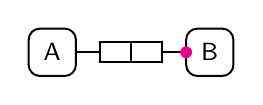
\begin{tikzpicture}
  \entity (A) {A};
  \entity at (2,0) {B} edge[mandatory]
          node[roles] (p) {} (A);
\end{tikzpicture}
\end{codeexample}
\end{stylekey}

\begin{stylekey}{required by}
This styles enables the |relationship| style and add a mandatory role dot at the end of a straight line.
\begin{codeexample}[]
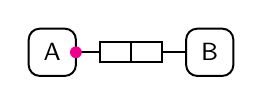
\begin{tikzpicture}
  \entity (A) {A};
  \entity at (2,0) {B} edge[required by]
          node[roles] (p) {} (A);
\end{tikzpicture}
\end{codeexample}
\end{stylekey}

\begin{stylekey}{both required}
\stylekeyheadline[]{both mandatory}
This styles enables the |relationship| style and adds mandatory role dots at both ends of a straight line.
\begin{codeexample}[]
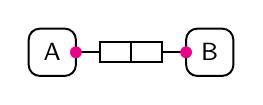
\begin{tikzpicture}
  \entity (A) {A};
  \entity at (2,0) {B} edge[both required]
          node[roles] (p) {} (A);
\end{tikzpicture}
\end{codeexample}
\end{stylekey}

\noindent To show that either of many roles is mandatory, you can add an \emph{inclusive-or} (\emph{disjunctive mandatory}) role constraint with |constraint=mandatory| as shown in section~\ref{sec:externalconstraints}. By default it is assumed that each entity or value must play at least some role. \emph{Independent object types} whose roles are collectively optional can be marked by an exclamation mark appended to its name. It is recommended not to include implied mandatory constraints unless they they refer to subtypes (section~\ref{sec:subtyping}).
\index{Independent object types}\index{Object types!Independent}


\subsection{External constraints}
\label{sec:externalconstraints}
External constraints span multiple roles that may come from different predicates. They are draw with circled symbol next to the roles, possibly linked to them with a dotted or dashed line (style |limits| and |limits to|).

\begin{stylekey}[\opt{\meta{constraint type}}]{constraint}
  This style sets the font to ORM style on constraint color (violet). If you provide a constraint type as key value, the current node is shaped as constraint circle and the symbol of the specified constraint type is drawn. The most common constraint types are |exclusive| (alias |x|) to indicate that populations of two or more role-sequences must be mutually exclusive, |mandatory| (alias |required|, |total|, and |or|) to indicate that each at least on of two more roles must be played by an object type, and |xor| (alias |partition|) to indicates that exactely one of two or more roles must be played by an object type. These constraints can also be used in subtyping (section~\ref{sec:subtyping}). The constraint type |unique| and |preferred unique| enforces combinations of object types that play a given set of roles to always be the same. The types |equal|, |subset|, and |supset| indicate that tuples of roles have to be equal, subset or superset compared to each other (|supset| is not included in standard ORM2). The constraint type is |misc| only draws the circle and can be used for custom constraints.
  % TODO: see more about rings and collections ...
\begin{codeexample}[]
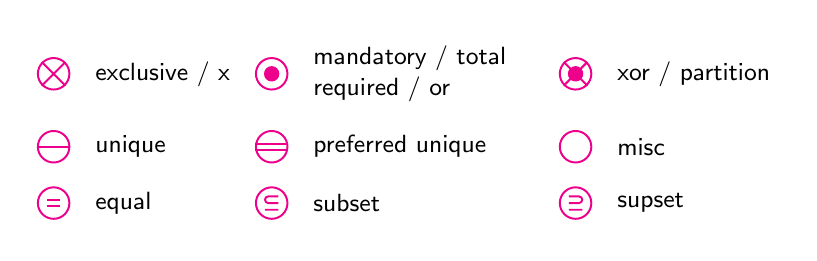
\begin{tikzpicture}[orm]
  \matrix[column sep=2mm, row sep=2mm]{
    \node[constraint=x]{};   & \node[right]{exclusive / x}; &
    \node[constraint=or]{};  & \node[right,text width=2.8cm]
                               {mandatory / total  required / or}; &
    \node[constraint=xor]{}; & \node[right]{xor / partition}; \\
    \node[constraint=unique] {}; & \node[right]{unique}; &
    \node[constraint=preferred unique]{};&\node[right]{preferred unique};&
    \node[constraint=misc]{}; & \node[right]{misc}; \\
    \node[constraint=equal] {}; & \node[right]{equal}; &
    \node[constraint=subset] {}; & \node[right]{subset}; &
    \node[constraint=supset] {}; & \node[right]{supset}; \\
  };
\end{tikzpicture}
\end{codeexample}
\end{stylekey}
\index{\texttt{custom} constraint}
\index{\texttt{x} constraint}
\index{\texttt{or} constraint}
\index{\texttt{xor} constraint}
\index{\texttt{mandatory} constraint}
\index{\texttt{required} constraint}
\index{\texttt{total} constraint}
\index{\texttt{partition} constraint}
\index{\texttt{unique} constraint}
\index{\texttt{preferred unique} constraint}
\index{\texttt{equal} constraint}
\index{\texttt{subset} constraint}
\index{\texttt{supset} constraint}


\begin{stylekey}{limits} % TODO: add optional parameter
  This style is to be used with lines that connect constraint circles and roles. It can also be used to link other kinds of constraints (for instance value constraints) to the entity, value, or role they belong to.
\begin{codeexample}[width=3cm]
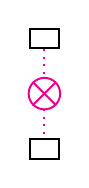
\begin{tikzpicture}
  \unary (r1) at (0,0) {};
  \unary (r2) at (0,-1.4) {};
  \draw[limits] (r1) to node[constraint=x] {} (r2);
\end{tikzpicture}
\end{codeexample}
  % TODO: example of subtyping constraints
\end{stylekey}

\begin{command}[]{limits}
This command is an abbreviation for |\draw[limits]| inside |{tikzpicture}|.
\end{command}

\begin{stylekey}{limits to}  % TODO: add optional parameter
This style is to be used with directed lines that connect constraint circles and roles. The line is drawn in the same style as |limits| but dashed and with an arrow tip of style \arrowtip{orm arrow} at the head.
\begin{codeexample}[width=3.4cm]
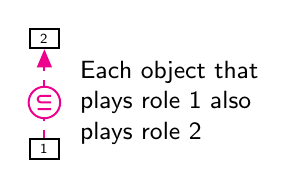
\begin{tikzpicture}[orm]
  \unary[index=2] (a) at (0,0) {};
  \unary[index=1] (b) at (0,-1.4) {};
  \draw[limits to] (b) -- (a) node[pos=.4,name=s]{};
  \node[constraint=subset] at (s) {};
  \node[right=2mm of s,text width=2.3cm] 
  {Each object that plays role 1 also plays role 2};
\end{tikzpicture}
\end{codeexample}
\end{stylekey}

\begin{command}[\marg{constraint type name}\marg{path code}]{constraintdeclare}
  This command declares a new constraint type. The \marg{path code} is passed to the |append after command| key to be drawn after the constraint circle. Unless you want to extend ORM you do not need to declare new constraint types.
\end{command}

\begin{command}[\marg{alias name}\marg{existing constraint type name}]{constraintdeclarealias}
  This command can be used to create an alias (another name) for an existing constraint type.
\end{command}

\begin{stylekey}{every constraint}
  This style is envoked at every constraint. You can change this style to change for instance the constraint color.
\end{stylekey}


\subsection{Ring Constraints}
\label{sec:ringconstraints}

A ring constraint can be applied to any two roles of a predicate that are played by the same object type (or the same supertype). Such constraints can also be viewed as properties of a binary relation or as properties of a directed graph. This package provides the following symbols to depict ring constraints. The graphical syntax of some symbols is slightly changed compared to the official ORM2 syntax and the two symbols for `asymmetric and intransitive', and for `symmetric and intransitive' have been omitted because of complexity.

% TODO: additional: transitive, tree
\begin{codeexample}[]
\centering
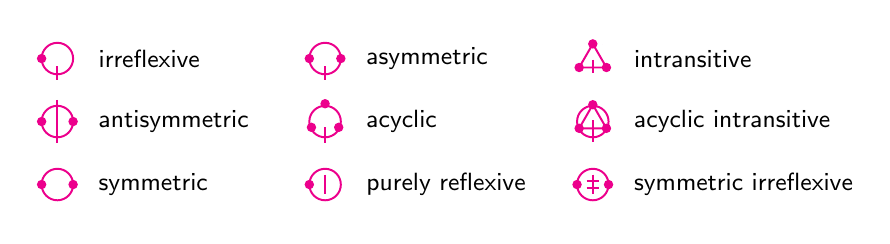
\begin{tikzpicture}[orm]
  \foreach \n/\s in {0/irreflexive,1/asymmetric,2/intransitive,
                     3/antisymmetric,4/acyclic,5/acyclic intransitive,
                     6/symmetric,7/purely reflexive,8/symmetric irreflexive}{
    \path ($mod(\n,3)*(3.4,0)-int(\n/3)*(0,0.8)$) node [constraint=\s] {}
         +(4mm,0) node[anchor=west] {\s}; };
\end{tikzpicture}
\end{codeexample}

\begin{codeexample}[width=2.5cm]
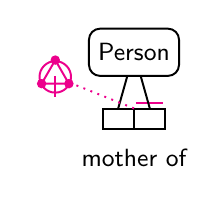
\begin{tikzpicture}[orm]
\entity (P) {Person};
\binary[below=of P,unique=2,label=below:mother of] (r) {};
\plays (P) to (r.one north) (P) to (r.two north);
\limits (r.north) to +(-1,0.4) node[constraint=acyclic intransitive]{};
\end{tikzpicture}
\end{codeexample}


\subsection{Number and Value Constraints}
Value constraints, cardinality constraints, and occurrence frequencies can simply be drawn beside the object type or role they refer to, optionally linked to with a dotted or dashed limitation line.

\noindent\textbf{Frequency Constraints} specify the number of times an object can play a role. Usually it is connected to the roles with a limtation line. % TODO: better syntax as pin

\begin{codeexample}[width=3cm]
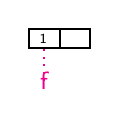
\begin{tikzpicture}
\binary[index=1:1] (b) {};
\limits (b.one south) -- +(0,-.4) node[constraint]{f};
\end{tikzpicture}
\end{codeexample}

\noindent A \textbf{Value constraint} indicates which values are allowed in an object type or role. It can be defined by declaring the set of possible values enclosed in curly brackets next to an object or role type. The command |\ormbraces| is a handy abbreviation to create curly brackets.
\index{value constraints}\index{constraints!values}

\begin{codeexample}[]
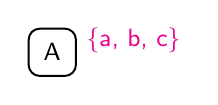
\begin{tikzpicture}
\entity (A) {A};
\node[constraint,anchor=north west,inner ysep=0] 
      at (A.north east) {\ormbraces{a, b, c}};
\end{tikzpicture}
\end{codeexample}

\noindent\textbf{Value comparision-constraints} are depicted by one of four comparision operators $<$, $\le$ (|le|), $>$, and $\ge$ (|ge|). The constraints are shown at a dashed arrow between two roles in the same way as |constraint=subset| and |constraint=supset| (but the value-comparision is between instances not between sets). Equality can be stated with |constraint=equal| which should not be confused with similar looking |constraint=purely reflexive|.
\index{value-comparision constraints}\index{constraints!value-comparision}
\index{\texttt{<} constraint}
\index{\texttt{>} constraint}
\index{\texttt{le} constraint}
\index{\texttt{ge} constraint}

\begin{codeexample}[]
\tikz \foreach \x/\s in {0/<,1/ge,2/>,3/le}{
  \draw[limits to] (\x,0) to (\x,1.2);
  \node[constraint=\s] at (\x,.5) {};
};
\end{codeexample}

\noindent\textbf{Cardinality constraints} are rarely included in ORM diagrams since the are often implied by other constraints. However you can explicitely say that each population of an object type or a role includes exactely, at most, or at least a given number of instances. This is done by adding a cardinality constraint next to the object or role. The hash sign (``\#'') stands for the cardinality. 
\index{cardinality constraints}\index{constraints!cardinality}

% TODO: Use text mode instead of math?
\begin{codeexample}[]
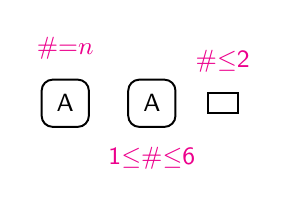
\begin{tikzpicture}[orm]
 \entity[label={[constraint]\#=$n$}] {A};
 \entity[label={[constraint]below:1$\leq$\#$\leq$6}]
        at (1.1,0) {A};
 \role[label={[constraint]\#$\leq$2}] at (2,0) {};
\end{tikzpicture}
\end{codeexample}



\subsection{Textual constraints}
\index{textual constraints}\index{constraints!textual}
Constraints not expressed by predefined graphical notation may be specified as textual rules. Textual rules can be displayed as footnotes with footnote numbers or signs that mark the involved elements in the diagram.

\begin{stylekey}[\opt{\meta{mark}}]{rule}
This key is to be used with nodes that contain textual rules. The optional \meta{mark} is shown as footnotes index left to the rule.
\begin{codeexample}[]
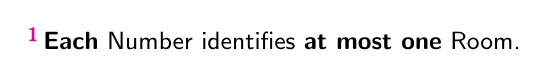
\begin{tikzpicture}
\node[rule=1] {{\ormbf Each} Number identifies {\ormbf at most one} Room.};
\end{tikzpicture}
\end{codeexample}
\end{stylekey}

\begin{command}[]{rules}
This command is an abbreviation for |\matrix[row sep=0mm,nodes={right}]| inside |{tikzpicture}|.
Matrices are useful to draw multiple textual rules below each other.

\begin{figure}[h]
\centering
\begin{codeexample}[]
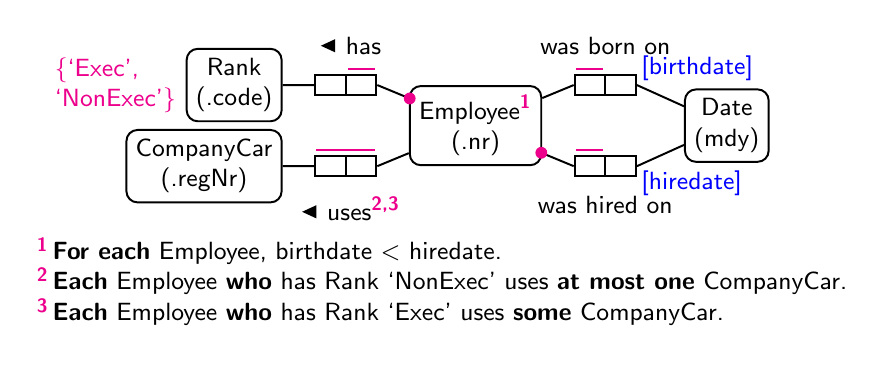
\begin{tikzpicture}[orm]
  \entity (E) {Employee\ormind{1}\\(.nr)};
  \binary[left=of E.north west,unique=2,label=\ormleft{has}] (h) {};
  \binary[left=of E.south west,unique=1-2,
          label=below:\ormleft{uses\ormind{2,3}}] (u) {};
  \entity[left=of h] (Rank) {Rank\\(.code)};
  \entity[left=of u] (Car) {CompanyCar\\(.regNr)};
  \node[constraint=text,align=left,anchor=east] at (Rank.west) 
      {\textbraceleft`Exec',\\`NonExec'\textbraceright};
  \plays[mandatory] (E) to (h.east);
  \plays (h) to (Rank) (E) to (u.east) (u) to (Car);
  \binary[right=of E.north east,unique,label=was born on] (b) {};
  \binary[right=of E.south east,unique,label=below:was hired on] (i) {};
  \entity[right=1.8 of E] (Date) {Date\\(mdy)};
  \plays[mandatory] (E) to (b.west) (E) to (i.west);
  \plays (b.east) to (Date) (i.east) to (Date);
  \node[role name,anchor=south west] at (b.east) {[birthdate]};
  \node[role name,anchor=north west] at (i.east) {[hiredate]};
  \rules at (-.4,-2) {
    \node[rule=1] {{\ormbf For each} Employee, birthdate $<$ hiredate.}; \\
    \node[rule=2] {
      {\ormbf Each} Employee {\ormbf who} has Rank `NonExec' uses 
      {\ormbf at most one} CompanyCar.};\\
    \node[rule=3] {
      {\ormbf Each} Employee {\ormbf who} has Rank `Exec' uses 
      {\ormbf some} CompanyCar.};\\
  };
\end{tikzpicture}
\end{codeexample}
\end{figure}
\end{command}

\section{Subtyping}
\label{sec:subtyping}

To draw type hierarchies you can use the tree syntax of \tikzname.
Euler diagrams are a less used alternative for simple type hierarchies.
% TODO: add Euler diagram example

\begin{stylekey}{subtype}
Draws a subtype relationship arrow from the supertype to the subtype.
\begin{figure}[h]
\centering
\begin{codeexample}[]
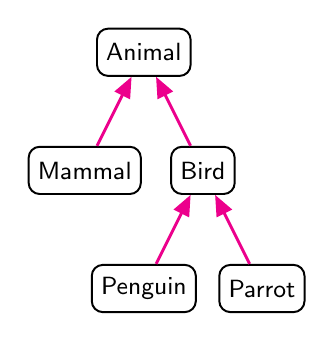
\begin{tikzpicture}[
  edge from parent/.style=subtype]
  \node[entity] {Animal}
    child {node[entity] {Mammal}}
    child {node[entity] {Bird}
      child {node[entity] {Penguin}}
      child {node[entity] {Parrot}}
    };
\end{tikzpicture}
\end{codeexample}
\end{figure}
\end{stylekey}

\begin{stylekey}{suptype}
Works in the same way as |subtype| but with reverse direction.
\begin{codeexample}[]
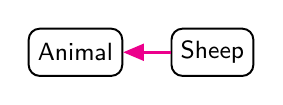
\begin{tikzpicture}
  \node[entity] (A) {Animal};
  \node[entity] (S) [right=6mm of A] {Sheep};
  \draw[suptype] (S) to (A);
\end{tikzpicture}
\end{codeexample}
\end{stylekey}

\noindent Multiple inheritance may require to select one path as primary.
You can distinguish primary and secondary subtypes by drawing the latter
with a dashed arrow (|subtype2| or |suptype2|).

\begin{stylekey}{subtype2}
\stylekeyheadline[]{suptype}
Draw secondary subtype/supertype relationship arrows.
\begin{codeexample}[]
\begin{tikzpicture}
  \node[entity] (A) {Animal};
  \node[entity] (P) [right=8mm of A] {Person};
  \draw[suptype2] (P) to (A);
\end{tikzpicture}
\end{codeexample}
\end{stylekey}


\noindent
Subtype constraints can be shown linked to the subtype arrrows:

\begin{figure}[h]
\centering
\begin{codeexample}[]
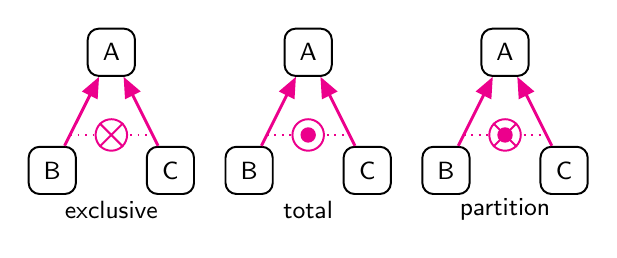
\begin{tikzpicture}[orm]
\foreach \c/\x in {exclusive/0,total/2.5,partition/5}{
  \entity (A) at (\x,0) {A} [edge from parent/.style=subtype]
    child {node [entity] (B) {B}} child {node [entity] (C) {C}};
  \limits ($(A)!.7!(B)$) to node[constraint=\c] {} ($(A)!.7!(C)$);
  \node at (\x,-2) {\c};
};
\end{tikzpicture}
\end{codeexample}
\end{figure}


\section{Additional Features}
\label{sec:additionalfeatures}
%\ldots partly no standard ORM2 \ldots

\subsection{Duplicated and implied parts of a model}
\label{sec:duplicatedandimplied}
Sometimes an object type or predicate is referred to without describing all its details because it is defined in an external model or because it is shown duplicated at some other place in the same model. To indicate such an external or duplicated object type or a predicate, a shadow is added to its shape. Alternatively ORM2 allows to add a circumflex ``\^{}'' to an object type's name. A different kind of redundancy are roles and constraints that deduce from other parts of the model. ORM2 includes the possibility to shade redundant roles. This is useful for instance to show conceptual pathes or join fact types that are normally excluded. Moreover ORM allows a \emph{zooming} on object types. This means that only objects and roles connected to a given object type are shown.

\begin{stylekey}{duplicated model}
This style modifies the styles |every orm object| and |every predicate| so all object types and predicates in the current scope get a shadow.
\begin{codeexample}[]
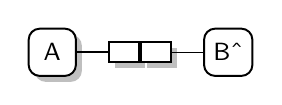
\begin{tikzpicture}[orm]
  \begin{scope}[duplicated model]
    \entity (A) {A};
    \node[role] (r1) [right=of A] {};
    \node[role] (r2) [right=0 of r1] {};
    \draw[relationship] (A) -- (r1);
  \end{scope}
  \entity (B) [right=of r2] {B\^{}};
  \draw[orm] (r2) -- (B);
\end{tikzpicture}
\end{codeexample}
\end{stylekey} % duplicated model

\begin{stylekey}{implied model}
  This style modifies the styles |every orm line| and |every orm object| in the current scope to draw all lines thin and all objects filled gray.
\begin{figure}[h]
\centering
\begin{codeexample}[]
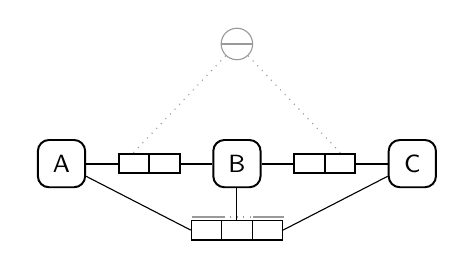
\begin{tikzpicture}
  \matrix[column sep=4mm] {
    \entity (A) {A}; & \binary (ab) {}; & \entity (B) {B}; &
    \binary (bc) {}; & \entity (C) {C}; \\ };
  \plays (A) -- (ab) -- (B) -- (bc) -- (C);
  \begin{scope}[implied model]
    \node[constraint=unique] (con) [above=of B] {};
    \limits (ab.one north) -- (con) -- (bc.two north);
    \ternary[unique=1-3,skip unique=2] (abc) [below=4mm of B] {};
    \plays (A) -- (abc.west); \plays (B) -- (abc); \plays (C) -- (abc.east);
  \end{scope}
\end{tikzpicture}
\end{codeexample}
\end{figure}
\end{stylekey}

% TODO command \implied{ ... } and \duplicated{ ... } ?

\begin{stylekey}{zoomed}
This styles visualizes an object type as {\emph zoomed} by using a thicker line.
\begin{codeexample}[]
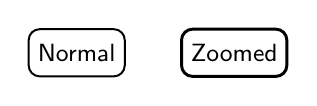
\begin{tikzpicture}
\entity at (0,0) {Normal};
\entity[zoomed] at (2,0) {Zoomed};
\end{tikzpicture}
\end{codeexample}
\end{stylekey}

\subsection{Macros for text layout} 
\label{sec:ormtext}
The following macros can be used both in \tikzname{} pictures or normal text:

\begin{command}{ormtext}
Sets the font to the same sans-serif variant which is used in ORM diagrams.
\end{command}

\begin{command}{ormbf}
Sets the font to a bold variant of |\ormtext|.
\end{command}

\begin{command}{ormc}
Sets the font to a |\ormtext| in constraint color.
\end{command}

\begin{command}[\marg{text}]{ormsup}
Puts some text in a superscript variant of |\ormtext|.
\end{command}

\begin{command}[\marg{text}]{ormsub}
Puts some text in a subscript variant of |\ormtext|.
\end{command}

\begin{command}[\marg{text}]{ormind}
Puts some text in a superscript variant of |\ormbf|.
\end{command}

\begin{command}[\marg{text}]{ormbraces}
Puts some text as |\ormtext| in braces.
\end{command}

\begin{codeexample}[]
\ormind{1}A {\ormtext Person} is not \ormbraces{0,1},~
{\ormc Male} {\ormbf or} {\ormtext Female}, \ormup{up}~
{\ormbf or} \ormleft{left} but \ormsub{queer}multi\ormsup{gender}!
\end{codeexample}


\section{Settings and Utilities}
\label{sec:generalstyles}

\begin{stylekey}{orm}
  This style sets the font and line width and the default node distance
\end{stylekey}

\begin{stylekey}{every orm line}
  This style is envoked by all styles of this package that draw lines. By default it sets the line width to 0.3mm.
\end{stylekey}

% \begin{stylekey}{every orm object}
% \end{stylekey}
% For this purpose (and for subtype arrows) this package defines the arrow tip \arrowtip{orm arrow}.
% TODO: document arrow tip \arrowtip{orm arrow}
% TODO: replace search path with |/orm/| instad of |/tikz/|.


\section*{Changes}

\begin{description}
  \item[\ormVersion, \ormDate]
    Unstable developer version (at Github)
  \item[0.1, January 25th, 2010]
    First release (at CTAN)
\end{description}

\ifappendix
  \bibliographystyle{alpha}
  \addcontentsline{toc}{section}{References}
  \bibliography{tkz-orm}
  \addcontentsline{toc}{section}{Index}
  \printindex
\fi

\end{document}
